\documentclass[../main.tex]{subfiles}
\graphicspath{{img},{img/ink},{ink}}

\begin{document}

\begin{tcolorbox}[
    width=\textwidth,
    height=\textheight,
    title=Phyphox: Schallgeschwindigkeit in Festkörpern,
    fonttitle=\Large,
    before title=\vspace{0.2cm}, after title=\vspace{0.2cm},
    colback=white,
    title filled=true, 
    colbacktitle=myorange,
    colframe=black,
    coltitle=black,
    ]

    \vspace{0.2cm}
    \textbf{Klassenstufe}: 9/10

    \vspace{0.4cm}

    \textbf{Fachlicher Bezug}: Schallgeschwindigkeit in Festkörpern, Eigenfrequenz

    \begin{minipage}[]{0.5\textwidth}
        \vspace{0.4cm} 
        \textbf{Material}:
        \begin{itemize}[noitemsep]
            \item Stativmaterial
            \item Eisenstange 1m
            \item Hammer
            \item Handy + Phyphox
        \end{itemize}

    \end{minipage}
    \hspace{1.4cm}
    \begin{minipage}[]{0.45\textwidth}
        \vspace{0.3cm}
        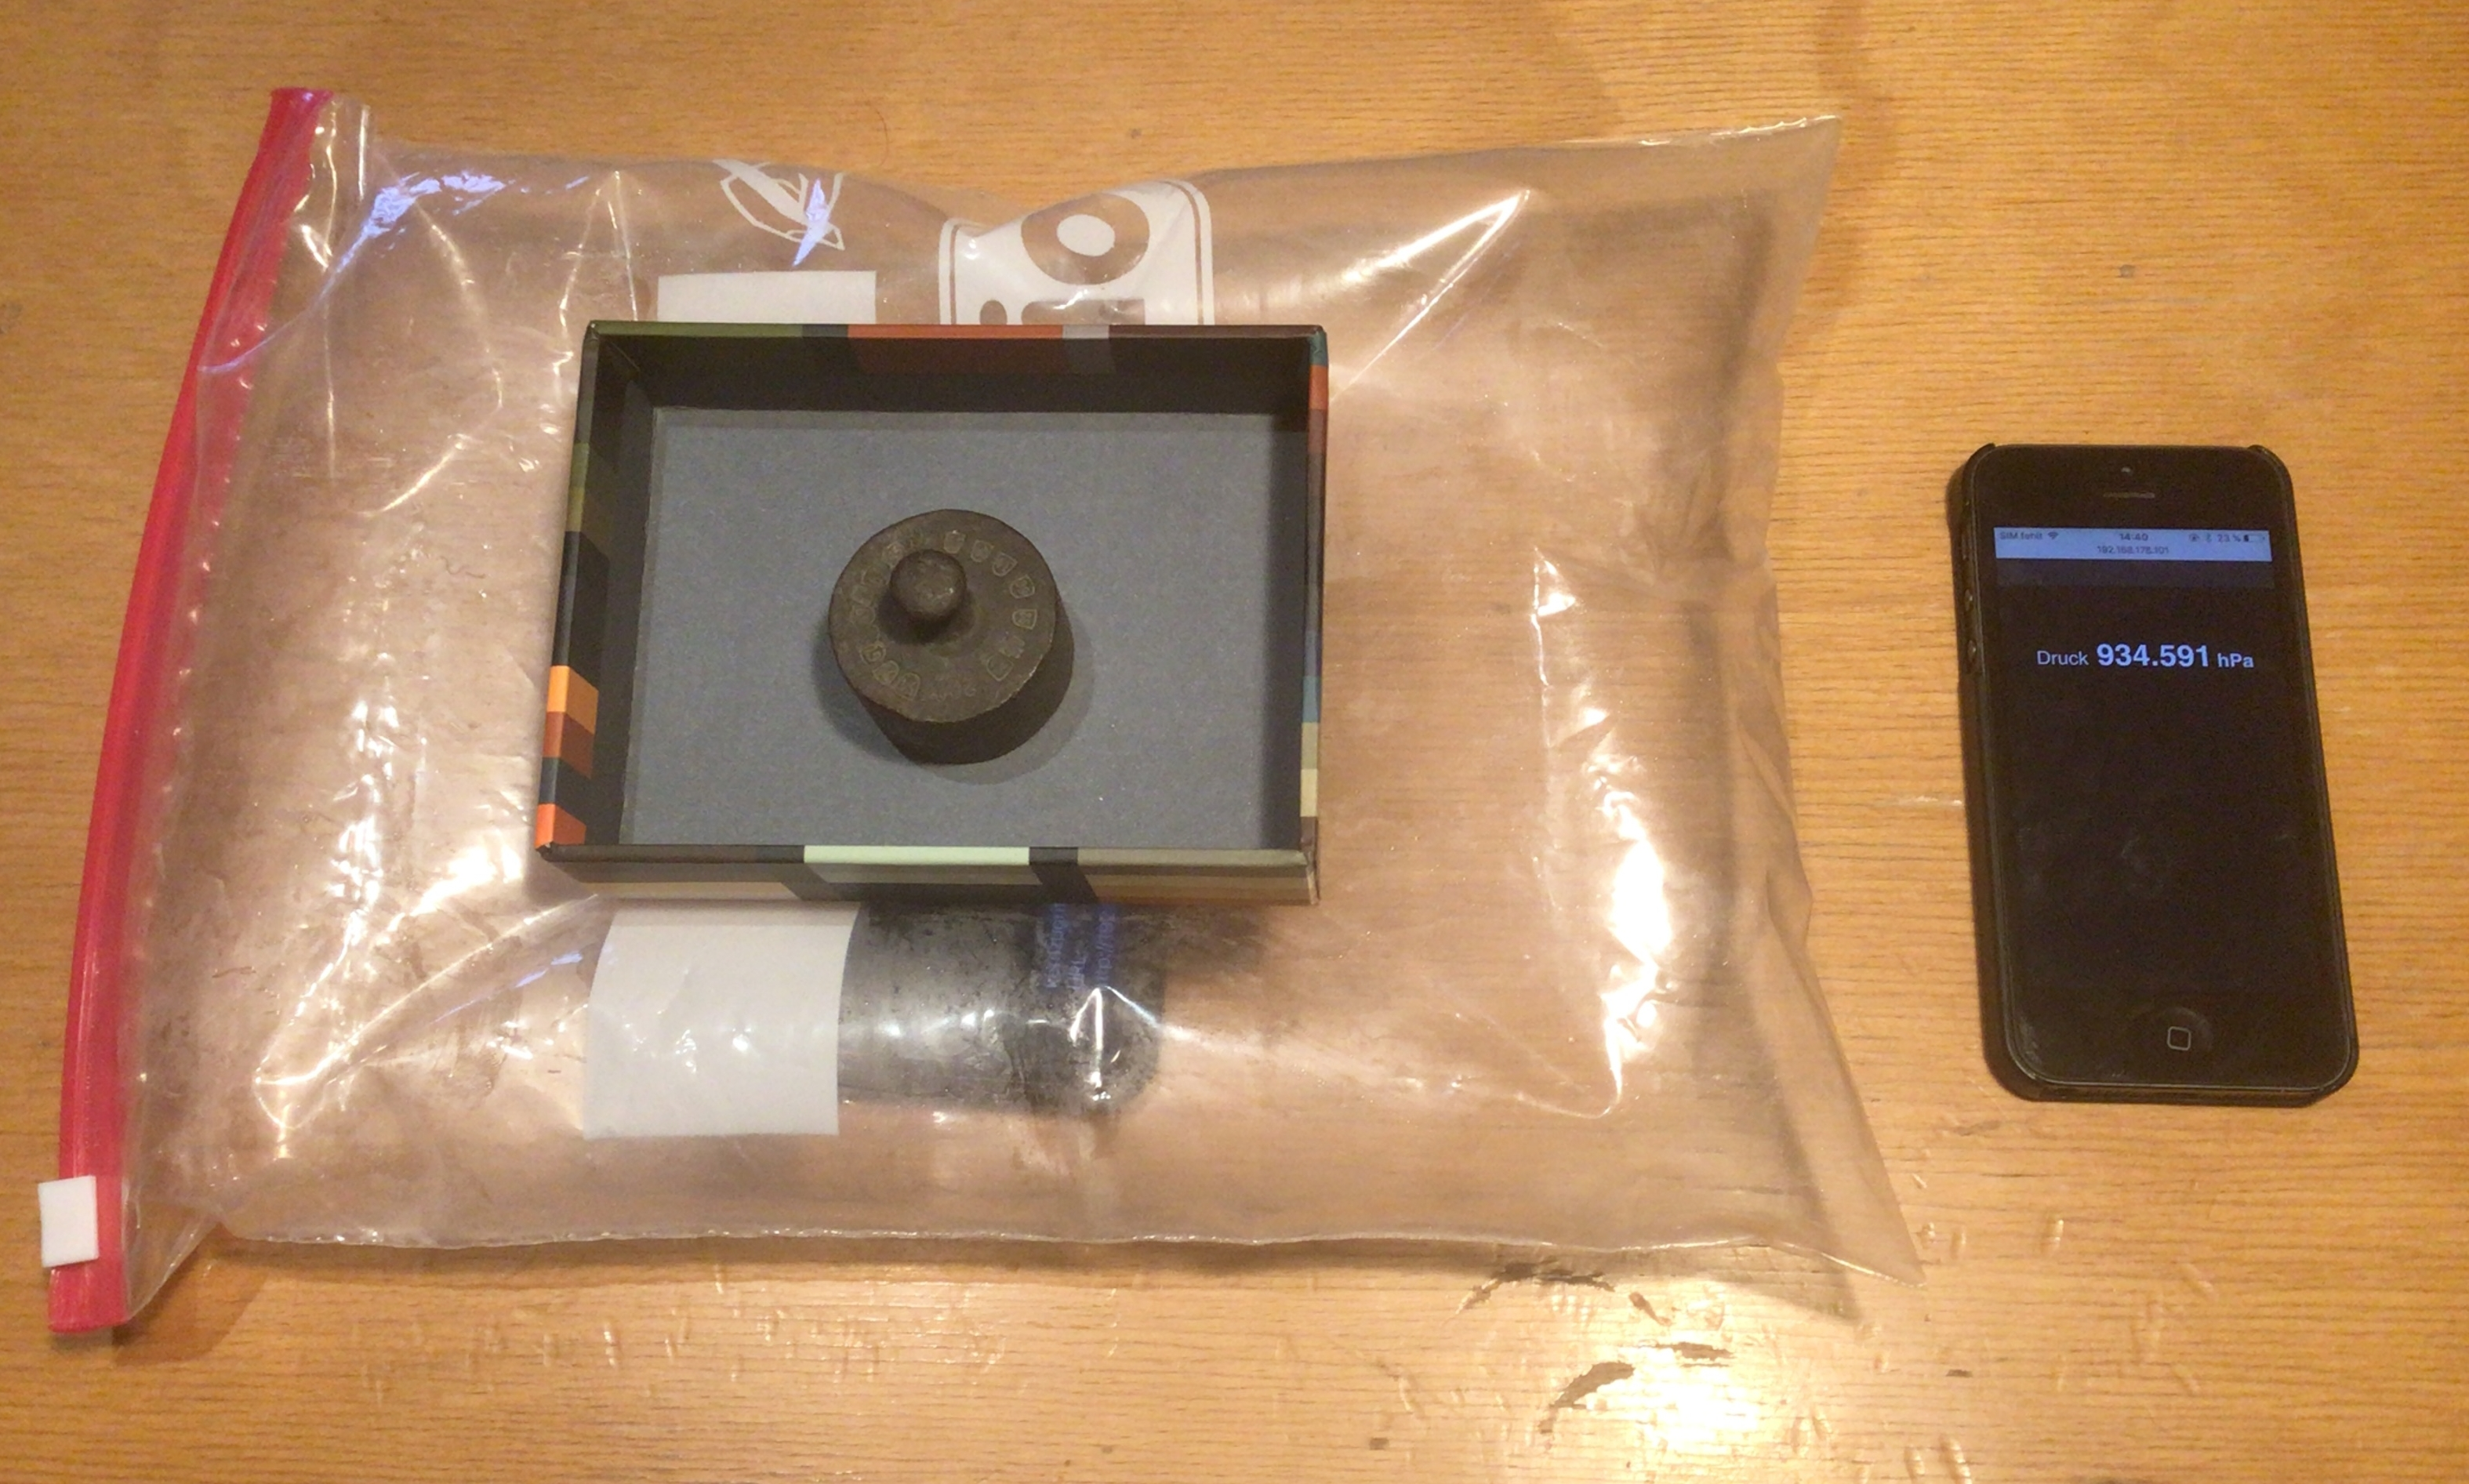
\includegraphics[width=0.9\textwidth]{img/versuchsaufbau}
    \end{minipage}

    \vspace{0.4cm}
    \textbf{Aufbau und Durchführung}: Ein Eisenstab mit einer Länge $L=1$ m wird zunächst bei $0,5\,$m und anschließend bei $0,25\,$m eingespannt. Das Handy wird in der Nähe platziert. In der Phyphox-App wird unter dem Reiter \glqq Akustik\grqq{} die Auswahl \glqq Audio Spektrum\grqq{} getroffen. Dort wird im Tab \glqq Spektrum\grqq{} der maximalen Wert der Frequenzspitze notiert, der beim Anschlagen des eingespannten Metallstabs für einen längeren Zeitraum (ca. 5 Sekunden) auftritt.

    \vspace{0.4cm}
    \textbf{Ergebnis}: Bei dem Aufbau handelt es sich um einen Stab mit freien Enden. Das Anschlagen führt zu einer Longitudinalwelle im Eisenstab. Bei passender Einspannung kann sich eine stehende Wellen mit entsprechender Eigenfrequenze $f_n$ (2) ausbilden. Dieser Zustand führt zu einem länger anhaltenden Ton, da das System ohne weitere äußere Anregung schwingen kann. Für die Wellenlänge $\lambda$ (1) gilt dabei

    \vspace{-3.3cm}
    \hspace{-0.7cm}
    \begin{minipage}[]{0.35\textwidth}
        \vspace{-0.5cm}
        \begin{align}
            \lambda &= \frac{2 \cdot L}{n} \\
            \Rightarrow \quad f_n &= n \cdot \frac{v_p}{2\cdot  L}\\[5pt]
            \Rightarrow \quad v_p &= \frac{2\cdot L \cdot f_n}{n}
        \end{align}
    \end{minipage}
    \hspace{0.2cm}
    \begin{minipage}[]{0.6\textwidth}
        \def\svgwidth{220pt}
        \input{ink/eigenfrequenz.pdf_tex}
    \end{minipage}

    \vspace{-3.2cm}
    \begin{minipage}[]{0.35\textwidth} 
        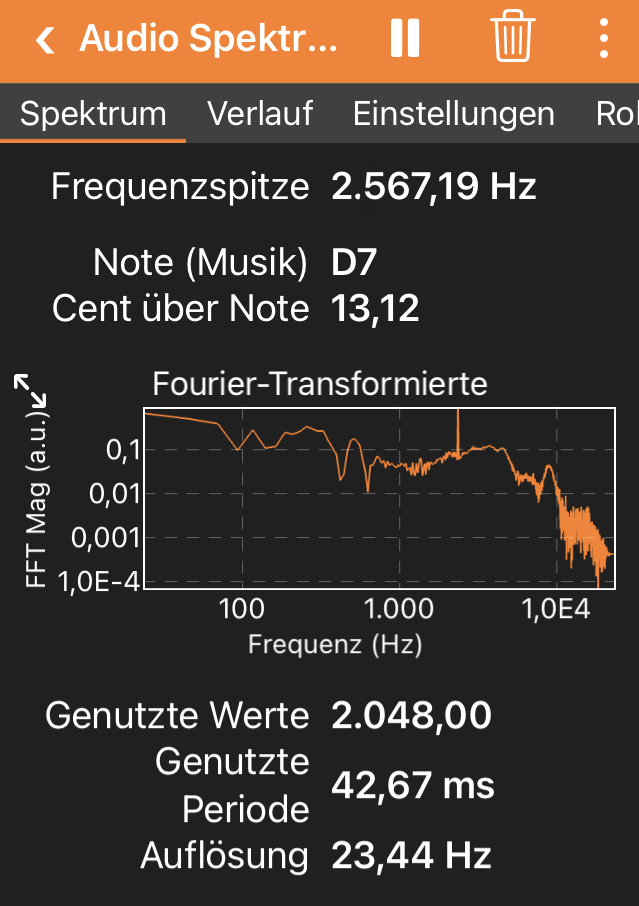
\includegraphics[width=1\textwidth]{img/n1}
    \end{minipage}
    \hspace{0.4cm}
    \begin{minipage}[]{0.6\textwidth}
        Für die Einspannung der Grundschwingung ($n=1$) erhält man $f_1=2567.19$ Hz.\\
        Für die Einspannung der 1. Oberschwingung ($n=2$) erhält man $f_2=5134.38$ Hz.\\
        Mit der Phasengeschwindikeit $v_p$ (3) kann sich dann auch der Schall $c_{\text{Eisen}}$ in der Eisenstange ausbreiten. Man erhält
        \begin{align*}
            c_{\text{Eisen}} = 5134.38 \, \frac{\text{m}}{\text{s}} 
        \end{align*}
    
        \vspace{0.4cm}
    \textbf{Didaktische Bemerkungen}: Das Experiment kann in verschiedenen Gruppen durchgeführt werden. Jede Gruppe kann ein anderes Material (z.B. Gewindestange/Stahl, Aluminium) untersuchen. Abschließend bietet sich der Vergleich mit Literaturwerten an. 
    \end{minipage}

\end{tcolorbox}


\end{document}
